\documentclass[11pt,a4paper]{ivoa}
\input tthdefs

\usepackage{todonotes}
\lstloadlanguages{XML,python}
\lstset{flexiblecolumns=true,tagstyle=\ttfamily, showstringspaces=False,
  basicstyle=\footnotesize}

\definecolor{termcolor}{rgb}{0.6,0.1,0.1}
\newcommand{\vocterm}[1]{\emph{\color{termcolor}#1}}
\newcommand{\vepitem}[1]{\emph{#1}}

\title{Vocabularies in the VO}

% see ivoatexDoc for what group names to use here
\ivoagroup{Semantics}

\author[https://wiki.ivoa.net/twiki/bin/view/IVOA/MarkusDemleitner]{Markus
Demleitner}
\author[https://wiki.ivoa.net/twiki/bin/view/IVOA/NormanGray]{Norman
Gray}
\author[https://wiki.ivoa.net/twiki/bin/view/IVOA/MarkTaylor]{Mark
Taylor}

\editor{Markus Demleitner}

\previousversion[http://ivoa.net/documents/Vocabularies/20190905/]
  {WD-20190905}
       

\begin{document}
\begin{abstract}
In this document, we discuss practices related to the use of RDF-based
vocabularies in the VO.  This primarily concerns the creation,
publication, and maintenance of vocabularies agreed upon within the IVOA.
To cover the wide range of use cases envisoned, we define three flavours
of such vocabularies: SKOS for informal knowledge organisation on the
one hand, and strict hierarchies of classes and properties on the other.
While the framework rests on the solid foundations of W3C RDF,
provisions are made to facilitate using IVOA vocabularies without
specific RDF tooling.
Non-normative appendices detail the current vocabulary-related tooling.
\end{abstract}


\section*{Acknowledgments}

While this is a complete rewrite of the specification how vocabularies
are treated in the VO, we gratefully acknowlegde the groundbreaking work
of the authors of version 1 of Vocabulary in the VO, S\'ebastien
Derriere, Alasdair Gray, Norman Gray, Frederic Hessmann, Tony Linde,
Andrea Preite Martinez, Rob Seaman, and Brian Thomas.

In particular, the vocabulary for datalink semantics done by Norman Gray
was formative for many aspects of what is specified here.

\section*{Conformance-related definitions}

The words ``MUST'', ``SHALL'', ``SHOULD'', ``MAY'', ``RECOMMENDED'', and
``OPTIONAL'' (in upper or lower case) used in this document are to be
interpreted as described in IETF standard RFC2119 \citep{std:RFC2119}.

The \emph{Virtual Observatory (VO)} is a
general term for a collection of federated resources that can be used
to conduct astronomical research, education, and outreach.
The \href{http://www.ivoa.net}{International
Virtual Observatory Alliance (IVOA)} is a global
collaboration of separately funded projects to develop standards and
infrastructure that enable VO applications.

\section{Introduction}

The W3C's Resource Description Framework RDF \citep{note:rdfprimer} is a powerful
and very generic means to represent, transmit, and reason on highly
structured, ``semantic'' information.  With both its power and
generality, however, comes a high complexity for consumers of this
information if no further conventions are in force.  Also, the generic
W3C standards understandably do not cover how semantic resources (e.g.,
vocabularies or ontologies) are to be managed, let alone developed
within organisations like the IVOA.

Based on a set of use cases (sect.~\ref{sect:usecases}) and requirements
(sect.~\ref{sect:requirements}), this standard will therefore define
conventions for
vocabularies based on either SKOS or RDFS in
sect.~\ref{sect:voccontent}.  Where these vocabularies -- and hence, in
particular, the permanent URIs of their RDF resources (``terms'') 
-- are managed by the
IVOA, they need to be reviewed and consensus be found.  A process to
ensure this is described in
sect.~\ref{sect:management}.  In order
to provide certain guarantees to clients, sect.~\ref{sect:deployment}
defines minimal standards for how IVOA-managed vocabularies must be made
available.  In addition, sect.~\ref{sect:withoutrdf} discusses how IVOA
vocabularies can be used without knowledge of RDF.

The non-normative appendices~\ref{app:tools} and \ref{app:curtech} 
describe the tooling
currently used or recommended for building and managing vocabularies in the
IVOA.


\subsection{Role within the VO Architecture}

\begin{figure}
\centering

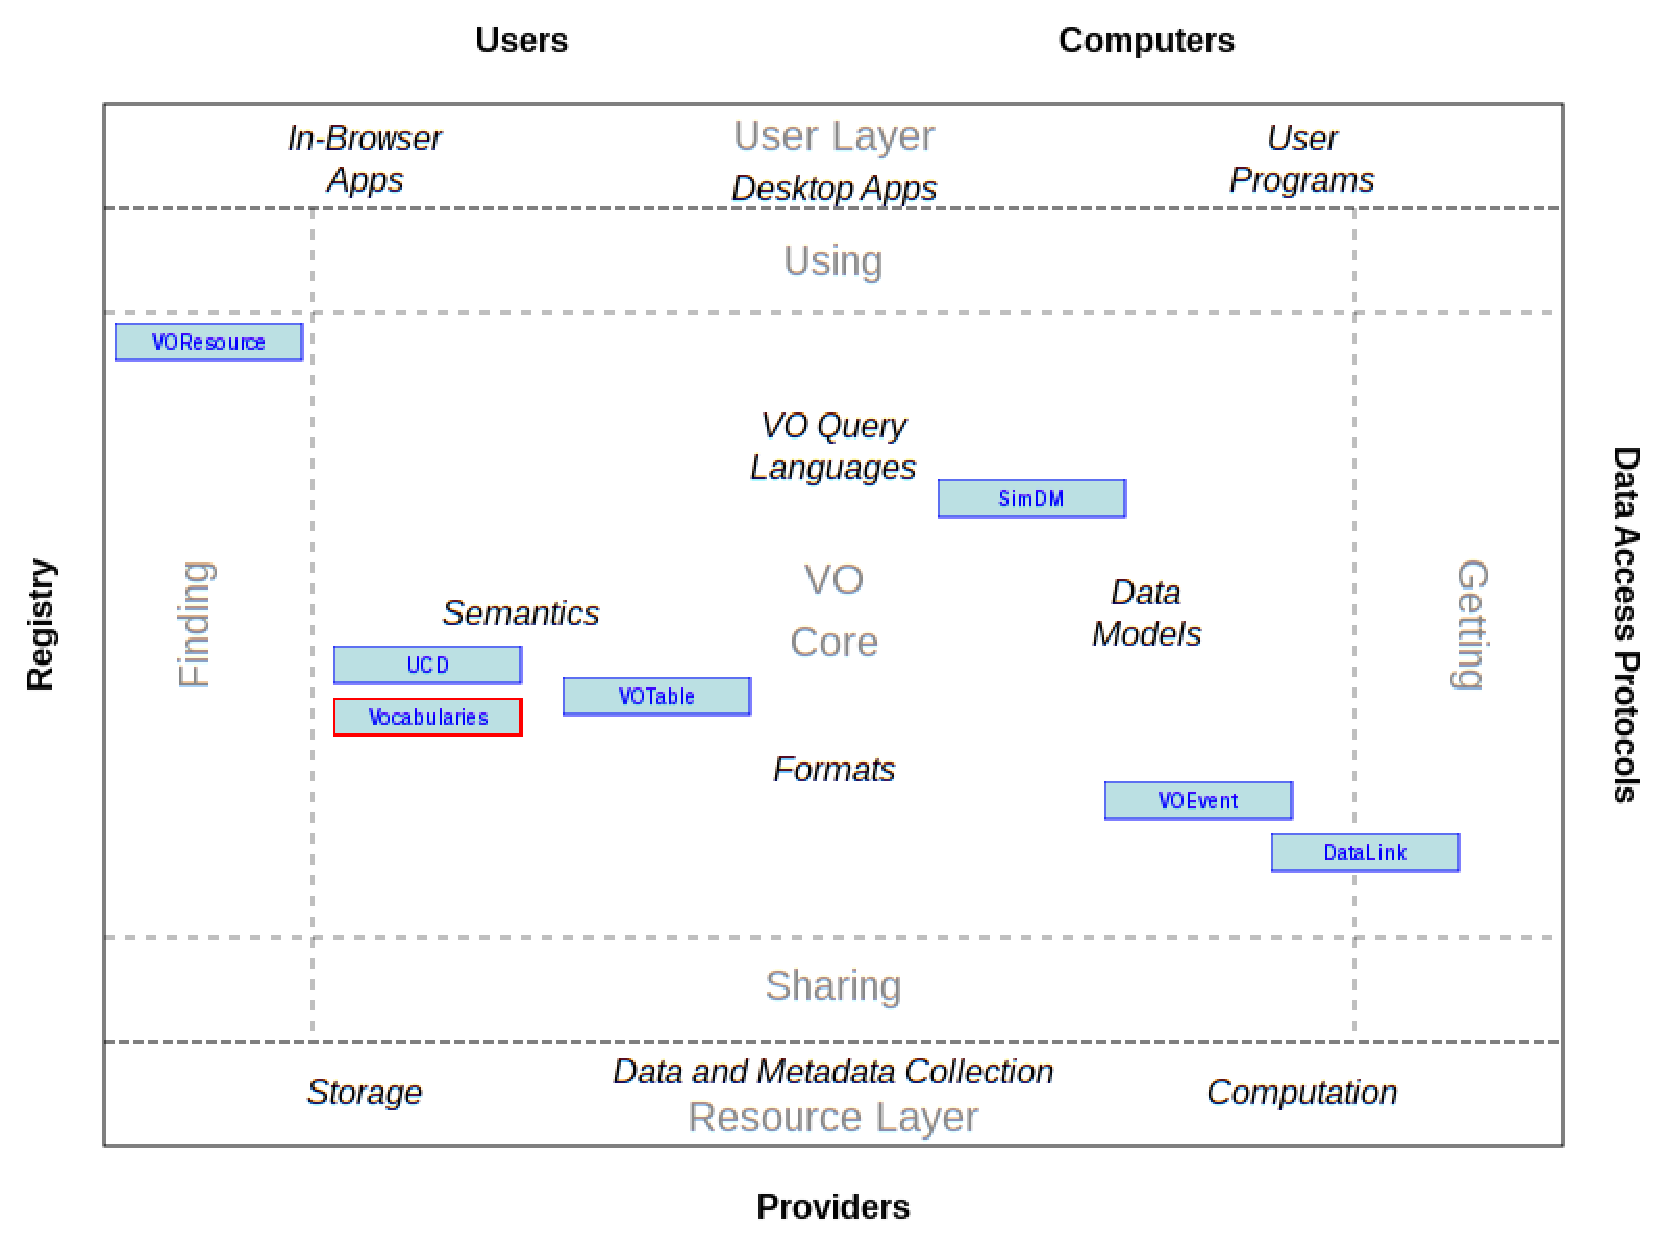
\includegraphics[width=0.9\textwidth]{role_diagram.pdf}
\caption{Architecture diagram for this document}
\label{fig:archdiag}
\end{figure}

Fig.~\ref{fig:archdiag} shows the role the Vocabularies in VO standard
plays within the IVOA architecture \citep{note:VOARCH}.

This standard provides the glue between several W3C standards and VO
standards that use them within the VO, including:

\begin{bigdescription}
\item[Datalink \citep{2015ivoa.spec.0617D}] Datalink includes a
vocabulary letting clients work out the kind of artefact a row pertains
to.

\item[VOResource \citep{2018ivoa.spec.0625P}] VOResource 1.1 comes with
several (rather flat) vocabularies enumerating, for instance, the types
of relationships between VO resources, their intended audiences, or
classes of actions performed on them.

\item[VOEvent \citep{2006ivoa.spec.1101S}] VOEvent defines \emph{Why}
and \emph{What} elements which, while not formally required to be drawn
from a specific vocabulary in version 1.11, certainly become much more
useful if they are.

\item[VOTable \citep{2019ivoa.spec.1021O}] VOTable, in its version 1.4,
introduces vocabularies for time scales and reference positions.

\item[SimDM \citep{2012ivoa.spec.0503L}] The Simulation Data Model has
several fields the values of which are required to be \vocterm{skos:narrower}
than certain top-level concepts; this includes the computational
methods employed, the physics simulated, or classes of objects
simulated.

\item[UCDs \citep{2007ivoa.spec.0402M}] UCDs are related to vocabularies in
that they provide machine-readable semantics.  Because the terms listed
in the document can be combined and have an underlying grammar, however,
they go beyond standard RDF.
\end{bigdescription}

\subsection{Relationship to Vocabularies in the VO Version 1}

Published in 2009, version 1.19 of the IVOA Recommendation on
Vocabularies in the VO had an outlook fairly different from the present
document: The big use case was VOEvent's Why and What, and so its focus
was on large, general-purpose vocabularies, of which several existed even
back then, while an overhaul of a thesaurus of general astronomical
terms approved by the IAU in 1993 was underway as part of IVOA's
activities.  Mapping between vocabularies maintained by different VO
and non-VO parties seemed to be the way to ensure interoperability and
therefore played a large role in the document.  Also, the use cases
called for ``soft'' relations, which is why the standard confined itself
to SKOS as the vocabulary formalism.

Since then, ``the'' large astronomy thesaurus is being maintained
outside of the IVOA (the UAT\footnote{\url{http://astrothesaurus.org}}),
and there is hope that its takeup will be sufficient to make mapping
between it and, say, legacy journal keyword systems an exercise general
clients will not have to perform.

Instead, in 2010, a fairly formal vocabulary of what
should be properties (in the RDF sense) rather than \vocterm{skos:Concept}-s
was required during the development of the datalink standard.  The
vocabulary was (and still is) small in comparison to, say, the UAT.  In
contrast to the expectations of Vocabularies~1, the plan had been that
most data providers would work with this small vocabulary, and terms
from external vocabularies would only be used as temporary stand-ins
until the consensus vocabulary was updated.  Of course, this required a
process for managing such vocabularies.  The lack of such a process
became even more noticeable when VOResource 1.1 and VOTable 1.4
introduced vocabularies of their own similar in size and scope to the
datalink vocabulary.

On the other hand, we are not aware of a single attempt to map
between different vocabularies in a VO context, and the SKOS versions of
some vocabularies that Vocabularies 1 declared as normative in its
section~4 were largely unused and have been unmaintained for a while now.

Since large parts of the original specification turned out to be
irrelevant or unsustainable as the VO ecosystem evolved, 
while some core requirements found later
were not addressed, it was decided to prepare a new major version of the
Vocabularies in the VO standard.

\subsection{Reading Guide}

We hope that software authors or annotators just wanting to consume IVOA
vocabularies or use them to annotate documents will be able to
do so after reading just section~\ref{sect:withoutrdf}.  In particular, no
deeper understanding of RDF should be necessary.

Persons intending to participate in vocabulary evolution should skim
sect.~\ref{sect:voccontent}, in particular the subsection on the kind of
vocabulary they want to modify, and must study
sect.~\ref{sect:management}.

Readers unfamiliar with RDF should read \citet{local:normanspaper} before
reading anything outside of section~\ref{sect:withoutrdf}.  
In particular, we assume familiarity with all RDF
terminology discussed there.  Concepts not covered by Gray's
essay will be informally introduced here.  Of course, the
underlying W3C standards are normative where applicable.



\subsection{Terminology, Conventions, Typography}

When we speak of \emph{term} here, that either means a \vocterm{skos:Concept}
in SKOS vocabularies, an \vocterm{rdfs:Class} in RDF class vocabularies,
and an \vocterm{rdf:Property} in RDF property vocabularies.  We also use
\emph{term} for ``the string after the hash character in
the RDF resource URI'', i.e., the machine-readable string typically used
in annotation.  It is rarely necessary to distinguish between the two
meanings.

We refer to classes and properties by CURIEs.  The prefixes in this
document correspond the the following URIs:

\begin{compactitem}
\item dc -- \url{http://purl.org/dc/terms/}
\item rdf -- \url{http://www.w3.org/1999/02/22-rdf-syntax-ns#}
\item rdfs -- \url{http://www.w3.org/2000/01/rdf-schema#}
\item owl -- \url{http://www.w3.org/2002/07/owl#}
\item skos -- \url{http://www.w3.org/2004/02/skos/core#}
\item ivoasem -- \url{http://www.ivoa.net/rdf/ivoasem#}
\end{compactitem}

Vocabulary terms are written in italics (e.g., \vocterm{rdfs:Class})
and, where supported, in a reddish hue.  As common in IVOA
specifications, XML element and attribute names are written in
typewriter italic (e.g., \xmlel{img}).

\section{Derivation of Requirements (Non-Normative)}

\subsection{Use Cases}
\label{sect:usecases}

The normative content of this document is guided by a set of
requirements derived from the following use cases.

\subsubsection{Controlled Vocabulary in VOResource}
\label{uc:simplevoc}

In VOResource, in certain use cases clients have to find services that
publish a given data collection.  This is effected by linking the resource
records for service and data with a
DataCite-compatible \vocterm{isServedBy} relationship.
Its concrete literal needs to be reliably defined in order to let
clients find such relationships by a simple string comparison in RegTAP
queries.

A related use case is that validators can flag errors (or at least
warnings) when resource records use terms that are not part of some
controlled vocabulary (e.g., content levels or types of events in a
resource's history).  Very typically, such out-of-vocabulary terms
indicate small oversights on the part of the resource record author that
will lead to hard-to-debug problems in data discovery.

\subsubsection{Controlled Vocabularies in VOTable}
\label{uc:votvoc}

VOTable 1.4 constrains two attributes of the TIMESYS elements 
-- reference positions and time
scales -- using vocabularies.  
While with time scales the situation is not fundamentally
different from the VOResource case discussed in
use case.~\ref{uc:simplevoc} -- a simple enumeration of agreed-upon strings
is enough to uniquely determine what operations need to be performed to
combine times given in different time scales --, the situation for
reference positions is probably different. There, even if a client does
not exactly know the location of, say, the Hubble Space Telescope at any
given time, several important use cases can already be satisfied if a
client knows that it is in lower Earth orbit (e.g., assuming a reference
position Geocenter and adjusting the systematic error estimates).  For
this, a client needs information of the type ``\vocterm{HST}
\vocterm{is-close-to} \vocterm{GEOCENTER\/}'' (or similar).

There is also another difference between this and at least the
VOResource relationship vocabulary from use case~\ref{uc:simplevoc}
in that the latter is property-like, as
in ``Resource-1 \vocterm{isServedBy} Resource-2\/''.  In constrast with
this, a time scale would be used like ``Time-coordinate
\vocterm{is-given-in}
\vocterm{TT\/}''.  In RDFS terminology, they are therefore better modelled
as classes rather than properties.

\subsubsection{Datalink Link Selection}
\label{uc:links}

In Datalink, clients receive a set of links
to pieces of information (e.g., previews, additional metadata,
progenitors, or
derived data) and need to present to the user only those items
relevant to the task at hand.  For instance, in a discovery phase, only
previews should be offered, while scientific exploitation would call for
cutout services, alternate formats, or derived data.  For debugging,
progenitors should be made accessible, and so on.

Operators of datalink services, on the other hand, want to be precise in
their annotation of datasets.  For instance, they may want to discern
among progenitors the raw image, a dark frame, and a flat field.  In all
these cases, clients should still be able to work out that such
artefacts are progenitors.

\subsubsection{VOEvent Filtering, Query Expansion}
\label{uc:filtering}

In VOEvent, an event stream can contain a classification of what the
observers believe was observed, for instance ``supernova Ia explosion''.
While an event stream from one project might provide a classification on
that level for some event, it might not (yet) be able to do that in
another event, and a different event stream might not be able to
distinguish between different sorts of supernovae at all.

In this situation, an event broker looking for supernovae of type Ia
will filter out anything not related to supernovae; however, since for
one reason or another a Ia supernova might only be tagged as supernova,
it will want to widen its filter somewhat, where some backend process
might prioritise events classified as Ia upstream over those only tagged
as a generic supernova, and those, again, over those tagged explicitly
as some different type of supernova.

Similar use cases exist, for instance, in the discovery of simulations
and possibly for subjects of VO resources.


\subsubsection{Vocabulary Updates in VOResource}
\label{uc:deprecation}

In VOResource 1.0, relationship types like \vocterm{served-by} or
\vocterm{service-for} were defined.  Later, DataCite defined equivalent
terms \vocterm{IsServedBy} and \vocterm{IsServiceFor}.  Arguably, the VO should,
as far as sensible, take up standards in the wider data management
community, and so VOResource 1.1 adopts the DataCite terms.  In a minor
version, it cannot forbid the old terms.  It can, however, say not only
``\vocterm{served-by\/} is the same as \vocterm{isServedBy\/}'' but also
``Use the latter term in preference to the former''.  If this information is
available machine-readably, validators can warn against the use of
deprecated terms and user interfaces can transparently replace 
deprecated terms with current ones.  This latter use case is is
already specified in RegTAP 1.1 \citep{2019ivoa.spec.1011D}.

Another use case in the context of VOResource and vocabulary updating
is the definition of content levels.  In VOResource 1.0, a list of
terms was adopted that was far too fine-grained in the area of public
outreach, distinguishing, for instance, ``Middle School'' from
``Secondary Education''; while this granularity was useful for the
original realm of the list of terms, in the VO it resulted in extremely
inhomogeneous annotation.  Obviously, persons employed in research
institutions can hardly be expected to assess needs and capabilities of
middle school versus elementary school educators.  Eventually, for
VOResource 1.1 a three-term list was drawn up and is now actually used.
To avoid a repetition of such an experience, we want to enable small
initial vocabularies easily extendable as new terms are actually needed
and the use of the existing terms is well understood.


\subsubsection{Discovering Meanings}
\label{uc:discovering}

Software developers or researchers want to work out
what some term mentioned ``means'' (where we are agnostic as to what
``means'' should mean here).  If the term URI alone is insufficient,
they can simply paste the resource URI of the term into a web browser
and read (at least) its description and perhaps find out even more using
relationships between terms.

\subsubsection{Simple Review Process}
\label{uc:simplereview}

As vocabularies evolve, new terms are being added to
vocabularies.  To facilitate their review and enable rapid uptake
of the proposed terms, it is desirable that new terms and even
new vocabularies are immediately visible to users and tools.
Note that since terms under review might be modified or removed later,
this use case is somewhat in conflict with the basic requirement
of stable vocabularies (i.e., a document valid once will not
become invalid later because of changes in vocabularies).

\subsubsection{Offline operation}
\label{uc:offline}

A system doing, say, coordinate transformations runs without an internet
connection but still needs to use semantic resources on frames and
reference positions (e.g., figure out that a given space probe is in L1
and use that as reference position).  To do that, it wants to use a
previously downloaded copy of the vocabulary.

\subsubsection{UAT in VOResource}
\label{uc:uat}

VOResource 1.1, in the description of the \xmlel{subject} element, says
that its content ``should be drawn from the Unified Astronomy Thesaurus''
(here: UAT).  This is intended to later facilitate interactive topic
navigation within the Registry or semantic expansion of Registry queries
(``include narrower terms'').


\subsection{Requirements}
\label{sect:requirements}

\subsubsection{Lists of Terms}
\label{req:lists}

We need to be able to represent simple lists of terms even for the most
basic use case~\ref{uc:simplevoc}.  As per
use case~\ref{uc:votvoc}, we will have to represent instances of both
\vocterm{rdf:Property} and \vocterm{rdfs:Class} (though not necessarily
in one vocabulary).

\subsubsection{Hierarchies of Terms}
\label{req:hierarchy}

Both use case~\ref{uc:links} and use case~\ref{uc:filtering} require a hierarchy
of terms, where clients can find wider and potentially narrower terms
relative to an original one.  There is a difference,
however: in the datalink use-case, strict \vocterm{is-a} relationships
are what clients need (e.g., ``give me all kinds of previews'').  In the
VOEvent case, however, a somewhat softer sort of hierarchy is required.
For instance, a filter for accretion disks might very well expand to
match both quasars and cataclysmic variables.  Hence, we want to
be able to represent strict class hierarchies as well as thesaurus-like
soft knowledge structures.

\subsubsection{Tree-like Hierarchies}
\label{req:tree}

Where we expect some sort of semi-formal inference to take place on the
vocabularies, the hierarchy should be a tree in order to facilitate
traversal and controlled query expansion.  In other words, outside of
SKOS we do not support multiple inheritance.  Use cases requiring
something equivalent would have to resort to supporting multiple terms 
on the annotation level.

\subsubsection{Consensus Vocabularies}
\label{req:consensus}

Essentially all our our use cases will be much easier to implement if
clients can work through simple string comparisons.  Therefore,
wherever feasible IVOA standards should build on IVOA-sanctioned,
consensus vocabularies.

\subsubsection{Deprecating Terms}
\label{req:deprecating}

While we believe at this point that terms once approved by the IVOA
should never disappear -- for instance, because validators might
otherwise flag previously valid instance documents as invalid --, use
case~\ref{uc:deprecation} shows that some way of declaring
deprecations must be forseen.

\subsubsection{Public Availability of Machine-Readable Vocabularies}
\label{req:machine}

In particular in use cases~\ref{uc:links} and \ref{uc:filtering},
clients can flexibly incorporate vocabulary updates without code
changes, perhaps even without re-deployment, if vocabularies are
available at constant, public URIs, where clients can retrieve them in
formats reasonably easy to parse.

Use case~\ref{uc:discovering} implies that at least one representation
of the vocabulary should be human-readable.

\subsubsection{Minimal Term Metadata}
\label{req:mtm}

To support use case~\ref{uc:discovering}, all terms in IVOA vocabularies
MUST come with a non-trivial description.

\subsubsection{Simple Cases do not Require RDF Tooling}
\label{req:nordf}

(Not derived from any specific use case).  Since libraries implementing
(some subset of) RDF tend to be rather massive and thus appear
unproportional when all a client wants is an up-to date list of terms
with their descriptions, at least the basic use cases must not require
specific RDF tooling.  Indeed, simple uses should not require an
understanding of RDF in the first place.


\subsubsection{Vocabulary Evolution}
\label{req:evolution}

Most use cases make it desirable that terms can be added to existing
vocabularies; this is very clear for the reference positions in
use case~\ref{uc:votvoc}, where new instruments would imply new
terms.  The history of content level annotation in VOResource mentioned
in use case~\ref{uc:deprecation} illustrates the desirability of a
simple process that invites standard authors to start with minimal
vocabularies, relying on later extensions.

\subsubsection{Preliminary Vocabularies and Terms}
\label{req:preliminary}

In use case~\ref{uc:simplereview}, it is desirable to admit
``preliminary'' vocabularies and terms.  For these, both humans
and machines must be able to discern a temporary status, and
their use implies that the general rule ``once valid, always
valid'' does not apply.  Validators and similar software could
then add notices to that effect in their outputs.

\subsubsection{Vocabulary Files are Usable Stand-Alone}
\label{req:standalone}

Vocabulary files need to be cacheable without applications having to
manage extra metadata (e.g., the URL from which the file was obtained)
in order to easily satisfy use case~\ref{uc:offline} (or other scenarios
in which vocabulary content cannot be retrieved from the IVOA
site for each session).

\subsubsection{Externally Curated Vocabularies and VO Tooling}
\label{req:external}

Regrettably, VOResource does not explain how use case~\ref{uc:uat} would
look like in actual documents, and the example given in the document
clearly does not use UAT concepts. 

The first difficulty in a straightforward uptake is that UAT URIs look
like \url{http://astrothesaurus.org/uat/1774}. Given that, should
publishers have such URIs in \xmlel{subject}?  Or should they rather use
just the last URI segment for conciseness?  Or perhaps the preferred
labels, in keeping with the style of existing subject content and its
use by clients (which typically look for natural language in subject),
even though the labels are not considered stable?

Regardless of how VOResource clarifies this matter, UAT artefacts (e.g.,
SKOS files), do not match some of our other requirements. In particular,
the human-readable URIs from \ref{req:lists}, the specific way we
satisfy \ref{req:machine}, and the non-RDF requirement \ref{req:nordf} are
not immediately satisfied by the UAT as distributed at the time of
writing.

For simple, uniform use of such externally curated vocabularies, it
should be possible to have some sort of endorsement process and then
distribute the vocabularies in a form compliant with this specification.
This will entail IVOA-specific concept URIs, and we must be able to
express that these resources have the same meaning as the ones
externally maintained.


\subsection{Non-Requirement}

This specification is not called ``Semantics in the VO'' or the like
because we do \emph{not} intend to prescribe ways to turn any VO
artefact into RDF triples.  Indeed, for many existing vocabularies, it
is left open what exactly the domain or range of properties might be or
what subject and predicate the classes or concepts should be used with.

This is partly because this would substantially complicate the
generation of vocabularies -- which would quickly turn into proper
ontologies --, partly because the information encoded by
the triples has traditionally been expressed using techniques developed
by the Data Models working group.

In particular with a view to later use in linked data scenarios,
vocabulary authors should neverthess take care that, given appropriate
properties or annotation tools, the vocabularies \emph{could} be used in
meaningful RDF triples.

Conversely, this specification is written with future ``deeper''
semantics in the VO in mind; tools restricting their operations to the ones
discussed here should not break when future specifications enrich
existing vocabularies towards full ontologies.


\section{Using IVOA Vocabularies without RDF Tooling}
\label{sect:withoutrdf}

RDF is a
powerful system for expressing a wide range of semantics and enriching
various documents with semantic information in a globally distributed
fashion.  Due to its generality, handling its artefacts is relatively
involved and in general requires special tooling, non-negligible
investment in understanding RDF, and non-trivial management of URIs and
prefix mappings.

To lower the bar for an adoption of IVOA vocabularies
[requirement~\ref{req:nordf}], they are given in
two formats usable without RDF tooling or, indeed, deeper knowledge of
RDF.  This section discusses these.

\subsection{Choosing Terms From IVOA Vocabularies}

Resource annotators can usually treat IVOA Vocabularies as simple lists
of (case-sensitive) strings with human-readable labels and definitions.  
These lists can be inspected with a simple web browser.

Each IVOA vocabulary has an associated URI starting with
\url{http://www.ivoa.net/rdf}.  Dereferencing that URI yields a list of
the vocabularies approved or under review.  

An individual vocabulary has a
URI like \url{http://www.ivoa.net/rdf/refposition}.  Dereferencing this URI
with a web browser (or, indeed, any user agent indicating it prefers
text/html media) redirects to a tabular representation of the vocabulary,
giving \emph{terms} -- i.e., the strings actually used in annotation --,
\emph{labels} -- i.e., strings that should be presented to humans instead of
the slightly formalised terms --, and \emph{descriptions}, which should
be sufficiently precise to allow someone with a certain amount
of domain expertise to decide whether a certain ``thing'' is or is not
covered by the term (or more precisely, the underlying concept).

Some terms may be marked as deprecated, in which case they should no
longer be used in new annotations.  In most cases, deprecated terms will
come with information about what to use instead.

Some terms may be marked as preliminary.  Such terms might disappear
without further notice.  Casual users should avoid the use of such
terms; if they find they want to use them, the semantics working group
requests notification over its mailing list, since such use is clearly
relevant to the term's adoption process.

Once a term is located within the HTML page, annotators can usually
directly use it in instance documents.  For instance, continuing the
refposition example, the string \texttt{BARYCENTER} found in the
vocabulary is directly used in VOTable's TIMESYS element.  

Some applications (Datalink being the prime example) instead use URIs
relative to the vocabulary URI.  In practical terms, this just means
that a hash sign is prepended to the term (e.g., \texttt{\#progenitor}).

This latter practice builds on the property of IVOA vocabularies that if
one adds the term as fragment to the vocabulary URI (e.g.,
\url{http://ivoa.net/rdf/refposition#BARYCENTER}), that URI is the full,
RDF-compliant resource identifier of the concept.  When used in
HTML-aware user agents (such as a web browser), dereferencing this URI
(i.e., opening it) will give the table of terms with the chosen term
highlighted.  How exactly this is represented depends on the user agent.


\subsection{Semantic Operations Without RDF Tooling}
\label{sect:desise}

Many VO components need a machine-readable representation of the
entire vocabulary, for instance in order to
(cf.~sect.~\ref{sect:usecases}):

\begin{compactitem}
\item display labels and descriptions for terms to users,
\item perform query expansion or similar exploitation of hierarchical
relationships, or
\item validate annotated instances for the use of correct and current
terms.
\end{compactitem}

To let VO programs perform such tasks with minimal technical overhead,
in addition to the RDF artefacts described in
sect.~\ref{sect:deployment}, IVOA vocabularies are also available in an
ad-hoc format called desise (``dead simple semantics'').  Clients can
obtain vocabularies in desise by retrieving the vocabulary URI with the
HTTP accept header set to \texttt{application/x-desise+json}.

What is returned is a JSON-encoded \citep{std:JSON} mapping (``object''
in JSON terms)
containing the following keys (all mandatory):

\begin{description}
\item[uri] The vocabulary URI.  All terms occurring in desise documents
can be turned into full, RDF-compliant resource URIs by prefixing them
with this URI and a hash character.
\item[flavour] The flavour of the vocabulary (can generally be ignored;
see sect.~\ref{sect:voccontent}).

\item[terms] A JSON object mapping the (machine-readable) terms to a
JSON object giving the term's properties as described below.
The keys in \textit{terms} are the strings used in
machine-readable data.
\end{description}

The JSON objects present as values in the terms object can have the
following keys:

\begin{description}
\item[label] (mandatory) 
A human-readable label for display purposes; clients should
always try to display this rather than the raw term.

\item[description] (mandatory) A human-readable definition of the underlying
concept.

\item[deprecated] present and mapped to a reserved value if the term is
deprecated and should no longer be used; validators will warn against
its use.

\item[preliminary] present and mapped to a reserved value if the term
is preliminary, meaning that in contrast to the other, ``eternal'' terms
it can disappear again; validators should qualify a validation as
preliminary if a document uses such a term.

\item[wider] (mandatory) A JSON array
of ``wider'' terms.  Most IVOA vocabularies are
tree-like, and for them, there is only up to one term in here, which
would be the the parent node, which is the hypernym of the current term.
In SKOS-flavoured vocabularies, multiple terms can be here, and the
meaning of ``wider'' is a bit less clear-cut.  The \textit{wider} list
is empty for top-level terms.

\item[narrower] (mandatory) A JSON array
of ``narrower'' terms.  In SKOS-flavoured
vocabularies, that is just a list of all terms that list the current
term as wider.  Otherwise, the vocabularies are tree-like and
\textit{narrower} is a list of all terms on the term's branch and below
it in the tree (it is the ``transitive closure of the inverse of
wider'').  This is much more easily understood in an example, which we
give below in the discussion on addressing use case~\ref{uc:links} below.
\end{description}

Note that, while \textit{wider} and \textit{narrower} are mandatory
keys, their values can of course be empty lists.

See appendix~\ref{app:desiseexample} for a example of a vocabulary
represented in desise.

For illustration, here are recipes to solve the various use cases in
Python, assuming \texttt{voc} contains a deserialised desise structure:

\paragraph{See if a term is in the vocabulary} (\ref{uc:simplevoc},
\ref{uc:votvoc})\\ \lstinline{term in voc["terms"]}

\paragraph{See if a term is deprecated} (\ref{uc:deprecation})\\
\lstinline{"deprecated" in voc["terms"][term]}

\paragraph{Find a human-readable label for a term}
(\ref{uc:discovering})\\
\lstinline{voc["terms"][term]["label"]}

\paragraph{Find a human-readable description for a term}
(\ref{uc:discovering})\\
\lstinline{voc["terms"][term]["description"]}

\paragraph{Find out if a term is preliminary} (\ref{uc:simplereview})\\
\lstinline{"preliminary" in voc["terms"][term]}

\paragraph{Query expansion: select branch} (in \ref{uc:links}, select all
progenitors, including flat fields, dark frames, etc)
\begin{lstlisting}[language=python]
base_term = "progenitor"
expanded_terms = set(
  [base_term]
  +voc["terms"][base_term]["narrower"])
is_match = datalink_row["semantics"][1:] in expanded_terms
\end{lstlisting}

\paragraph{SKOS-type query expansion by neighbouring terms}
(\ref{uc:filtering})
\begin{lstlisting}[language=python]
assert voc["flavour"]=="SKOS"
expanded_terms = set(
  [base_term]
  +voc["terms"][base_term]["narrower"]
  +voc["terms"][base_term]["wider"])
is_match = keyword_found in expanded_terms
\end{lstlisting}


\section{Vocabulary Content}
\label{sect:voccontent}

IVOA vocabularies MUST be based on W3C's Resource Description Framework.
Details on required serialisations are given in
sect.~\ref{sect:deployment}.  This section deals with what kinds of
statements users of IVOA vocabularies SHOULD evaluate to ensure
interoperability.   Statements of other types are legal in IVOA
vocabularies but are not expected to be interpreted interoperably.
Clients MAY ignore them.

In IVOA vocabularies, the concept URI MUST begin with
\url{http://www.ivoa.net/rdf}\footnote{In retrospect, the unnecessary
``www'' in this URI is somewhat regrettable, but existing vocabularies
have used URIs including it, and it seems a small price to pay for
having uniform URIs}.  It is recommended to not introduce
additional hierarchy levels, i.e., vocabulary URIs SHOULD be direct children
of \texttt{rdf}\footnote{Some existing vocabularies do not follow this
rule; since vocabulary URI changes will break certain usage scenarios,
their URIs are still retained.}.

Since all vocabularies specified here are
single-file, the full term (i.e., RDF resource) 
URI is formed by appending a hash sign
and a fragment identifier.  In IVOA vocabularies, this fragment
identifier MUST consist of ASCII letters, numbers, underscores and
dashes exclusively [for requirement~\ref{req:machine}].

The fragment identifiers in the vocabulary URIs SHOULD be
human-readable, usually by suitably contracting the
preferred label.  In the IVOA, we do \emph{not} use natural
language-neutral concept identifiers but instead expect that domain
experts will already have an impression of a term's meaning from looking
at its URI.

In this specification, we distinguish three different ``flavours'' of
vocabularies.  Each covers a particular domain of problems and is
therefore subject to different requirements.
Although the requirements are largely non-contradicting, each vocabulary must
be clearly identified as \emph{either} giving SKOS concepts, RDFS
classes or RDF properties so clients know how to extract word lists and
hierarchies; see sect.~\ref{sect:genprop}
for details.


\subsection{SKOS Vocabularies}
\label{sect:skosvoc}

SKOS vocabularies should be used where terms are organised 
in informal (i.e., non necessarily strict is-a)
hierarchies.  The classic use case here is query expansion, where, for
instance, a search for ``AGN'' might be expanded to include matches for
``accretion disk'' (under certain circumstances).

The terms in SKOS vocabularies have the RDF type \vocterm{skos:Concept}.

\subsubsection{Properties in SKOS Vocabularies}
\label{sect:skosvoc-prop}

IVOA SKOS vocabularies use the following properties:

\begin{itemize}
\item \vocterm{skos:broader} -- interpreted in the standard SKOS sense.
The reverse property, \vocterm{skos:narrower}, MAY be given, but clients
MUST NOT depend on their presence [this satisifies
requirement~\ref{req:hierarchy}].

\item \vocterm{skos:prefLabel} -- all concepts MUST have an
English-language preferred label, which is an RDF plain literal [by
requirement~\ref{req:mtm}].  No RDF language label is allowed on the
literal, and only one preferred label is permitted
[these help requirement~\ref{req:nordf}].

\item \vocterm{skos:definition} -- all concepts MUST have a non-trivial
English-language definition.  It is obviously impossible to define
``non-trivial'' in a rigorous way; a suggested criterion is that a
domain expert would, given the definition, presumably arrive at a
similar preferred label, and recursive definitions (i.e., those using
the label itself) should be avoided whenever possible.  Definitions in
non-English languages are not permitted, and only one definition is
permitted [again, this helps requirement~\ref{req:mtm}].

\item \vocterm{skos:exactMatch} -- for externally managed vocabularies
the IVOA has endorsed (see sect.~\ref{sect:externally-managed}), this
property links the IVOA term (subject) to the external RDF resource
(object).

\item General properties discussed in \ref{sect:genprop} [this is
for requirements~\ref{req:deprecating} and
\ref{req:preliminary}].  The \vocterm{ivoasem:vocflavour} of these
vocabularies is \verb|SKOS|.
\end{itemize}

This specification does not include requirements on the use or the
interpretation of \vocterm{skos:related}, 
\vocterm{skos:closeMatch}, \vocterm{skos:broadMatch},
\vocterm{skos:narrowMatch}, \vocterm{skos:ConceptScheme},
\vocterm{skos:inScheme}, \vocterm{skos:hasTopconcept},
\vocterm{skos:altLabel}, and \vocterm{skos:hiddenLabel}. If use cases
are found that require those, this specification will be amended.  Until
then, vocabulary authors SHOULD NOT use them in order to avoid creating
practices that might conflict with later usage patterns.

This specification does not include requirements on the use or the
interpretation of the transitive SKOS properties
(\vocterm{skos:broaderTransitive}, \vocterm{skos:narrowerTransitive}).
At this point, we believe that applications requiring this type of
reasoning-friendly semantics should preferably use RDF class
vocabularies.

\subsubsection{Example (non-normative)}

Here is a term from a SKOS vocabulary conforming to this specification
in RDF/XML serialisation:

\begin{lstlisting}[language=XML]
<skos:Concept rdf:about="http://ivoa.net/rdf/AstronomicalObjects#AGN">
  <skos:prefLabel>AGN</skos:prefLabel>
  <skos:definition>A compact object in the center of a galaxy showing 
    unusual emission ("active galactic nucleus").</skos:definition>
  <skos:broader rdf:resource
    ="http://ivoa.net/rdf/theory/AstronomicalObjects#OpticalSource"/>
  <skos:broader rdf:resource
    ="http://ivoa.net/rdf/theory/AstronomicalObjects#CompoundObject"/>
</skos:Concept>
\end{lstlisting}

\subsection{RDF Properties Vocabularies}
\label{sect:refpropvoc}

RDF properties vocabularies should be used when the terms in the
vocabulary are mainly used to state
relationships between entities that can sensibly be imagined as
resources in the RDF sense.  Such terms would naturally be used as
predicates in RDF triples.  Obvious examples might be something
like is-progenitor-for in a provenance chain or, indeed, the special
properties for IVOA vocabularies introduced in sect.~\ref{sect:genprop}.


The terms in RDF Properties vocabularies have the RDF type 
\vocterm{rdf:Property}.

\subsubsection{Properties in RDF Properties Vocabularies}
\label{sect:propvoc-prop}

IVOA RDF properties vocabularies use the following properties (where
not specified, the requirements considered essentially match those in
sect.~\ref{sect:skosvoc-prop}):

\begin{itemize}
\item \vocterm{rdfs:label} -- all terms MUST have an English-language
label, and clients should prefer it over the fragment in the
term URI for presentation purposes.  Only
one such label is permitted.

\item \vocterm{rdfs:comment} -- all concepts MUST have a non-trivial
English-language comment serving as a human-oriented definition of the
term.  The considerations for \vocterm{skos:definition} in
sect.~\ref{sect:skosvoc-prop} apply.  As for those, only one
\vocterm{rdfs:comment} per term is allowed.

\item \vocterm{rdfs:subPropertyOf} -- interpreted as in RDFS to induce
the hierarchy of terms; a term MUST NOT appear as subject of more than
one \vocterm{rdfs:subPropertyOf} triple (i.e., the hierarchy is a tree).

\item General properties discussed in sect.~\ref{sect:genprop}.  
The \vocterm{ivoasem:vocflavour} of these vocabularies is 
\verb|RDF Property|.

\end{itemize}

\subsubsection{Example (non-normative)}
\label{sect:rdfpxex}

\begin{lstlisting}[language=XML]
<rdf:Property rdf:about
  ="http://www.ivoa.net/rdf/datalink/core#preview-image">
    <rdfs:comment>preview of the data as a 2-dimensional 
      image</rdfs:comment>
    <rdfs:label>Image preview</rdfs:label>
    <rdfs:subPropertyOf rdf:resource
      ="http://www.ivoa.net/rdf/datalink/core#preview"/>
</rdf:Property>
\end{lstlisting}


\subsection{RDF Class Vocabularies}

RDF class vocabularies should be used when the terms in the vocabulary
are reasonably class-like, i.e., would usually be either subjects or
objects in RDF triples.  As opposed to SKOS vocabularies, the hierarchy
implied is strict in the sense of \vocterm{rdfs:subClassOf}
-- roughly, that statements true for a wider term must be true
a more specialised term, too.  This lets clients confidently perform
inferences.

For instance, coordinates in the FK4 reference frame are equatorial, and
thus even a client unfamiliar with the FK4 frame as such can confidently
infer that the coordinates are right ascension and declination, and that
right ascensions increase eastwards.  Reasoning of this type is
impossible within a SKOS vocabulary.

The terms in RDF Class vocabularies have the RDF type 
\vocterm{rdfs:Class}.

\subsubsection{Properties in RDF Class Vocabularies}
\label{sect:classvoc-prop}

IVOA RDF class vocabularies use the following properties:

\begin{itemize}
\item \vocterm{rdfs:label} -- all terms MUST have an English-language
label, and clients should prefer it over the term (the fragment of the
term URI) for presentation purposes.  Only
one such label is permitted.

\item \vocterm{rdfs:comment} -- all concepts MUST have a non-trivial
English-language comment serving as a human-oriented definition of the
term.  The considerations for \vocterm{skos:definition} in
sect.~\ref{sect:skosvoc-prop} apply.  As for those, only one
\vocterm{rdfs:comment} per term is allowed.

\item \vocterm{rdfs:subClassOf} -- interpreted as in RDFS to induce
the hierarchy of terms; a term MUST NOT appear as subject of more than
one \vocterm{rdfs:subClassOf} triple (i.e., the hierarchy is a tree).

\item General properties discussed in \ref{sect:genprop}.
The \vocterm{ivoasem:vocflavour} of these vocabularies is 
\verb|RDF Class|.
\end{itemize}

\subsubsection{Example (non-normative)}

Here is a term from an RDF class vocabulary conforming to this
specification in RDF/XML serialisation:

\begin{lstlisting}[language=XML]
<rdfs:Class rdf:about="http://www.ivoa.net/rdf/refframe#FK5">
    <rdfs:comment>
      Positions based on the 5th Fundamental Katalog. If no equinox is
      [...]
    </rdfs:comment>
    <rdfs:label>FK5</rdfs:label>
    <rdfs:subClassOf rdf:resource
      ="http://www.ivoa.net/rdf/refframe#EQUATORIAL"/>
</rdfs:Class>
\end{lstlisting}

\subsection{General Properties}
\label{sect:genprop}

To cover requirements~\ref{req:deprecating} and
\ref{req:preliminary} and to facilitate the handling of vocabularies not
directly retrieved via HTTP (which means that the application may not
know the vocabulary URI a priori; cf.~requirement~\ref{req:standalone}), 
the Semantics WG defines some
properties of its own in the vocabulary
\url{http://www.ivoa.net/rdf/ivoasem}.  The following properties may be
used in all three vocabulary flavours:

\begin{itemize}
\item \vocterm{dc:created} -- IVOA vocabularies MUST include exactly one
triple with the vocabulary as subject and a predicate
\vocterm{dc:created}.  The object is the datestamp of the vocabulary in
YYYY-MM-DD format.  Clients may only use this for debugging and similar
purposes.

\item \vocterm{ivoasem:vocflavour} -- IVOA vocabularies MUST include
exactly one triple with the vocabulary as subject and a string literal
specifying the kind of vocabulary as per this specification.  The
``General properties'' bullet points of sects.~\ref{sect:skosvoc-prop}
(\verb|SKOS|), \ref{sect:propvoc-prop} (\verb|RDF Property|), and
\ref{sect:classvoc-prop} (\verb|RDF Class|) define what strings may occur
here.

\item \vocterm{ivoasem:preliminary} -- this property indicates
that a term is preliminary and might disappear from the
vocabulary without warning.  The object of triples using it
is a blank node.  Validators need not warn against the use
of preliminary terms, but as they encounter them, they SHOULD
qualify their validation to the effect that it is temporary.

\item \vocterm{ivoasem:deprecated} -- this property indicates
that a term is deprecated.  The object of triples using it 
is a blank node.  Validators SHOULD issue warnings if such terms
are encountered.

\item \vocterm{ivoasem:useInstead} -- for a deprecated term, the
objects of RDF triples using this property indicate
which terms should be
used instead of the deprecated one.

\end{itemize}

\subsubsection{Example (non-normative)}

The following snippets show RDF/XML triples using the common terms,
taken from the existing relationship\_type vocabulary; the notation
\verb|__| as a blank node is an implementation detail and must not be
relied upon.  In general, where ivoasem properties take blank nodes as
objects, clients should normally just ignore the objects.

\begin{lstlisting}[language=XML]
<rdf:Description rdf:about
    ="http://www.ivoa.net/rdf/voresource/relationship_type">
  <dc:created>2016-08-17</dc:created>
</rdf:Description>
<rdf:Description rdf:about
    ="http://www.ivoa.net/rdf/voresource/relationship_type">
  <ivoasem:vocflavour>RDF Property</ivoasem:vocflavour>
</rdf:Description>
<rdf:Description rdf:about
    ="http://www.ivoa.net/rdf/voresource/relationship_type#IsPartOf">
  <ivoasem:preliminary rdf:resource=
    "http://www.ivoa.net/rdf/voresource/relationship_type#__"/>
</rdf:Description>
<rdf:Description rdf:about
    ="http://www.ivoa.net/rdf/voresource/relationship_type#derived-from">
  <ivoasem:deprecated rdf:resource
    ="http://www.ivoa.net/rdf/voresource/relationship_type#__"/>
  <ivoasem:useInstead rdf:resource
    ="http://www.ivoa.net/rdf/voresource/relationship_type#IsDerivedFrom"/>
</rdf:Description>
\end{lstlisting}


\section{Vocabulary Management}
\label{sect:management}

This section discusses the processes in which new vocabularies can be
defined and how vocabulary updates are performed in way
that ensures community participation and at least a minimal level of consensus.
In the following, the phrase ``chair of the Semantics WG'' is understood
to mean ``chair or vice-chair of the Semantics WG''; in the unlikely
situation that chair and vice-chair dissent, the resolution of the
problem is up to the TCG chair.


\subsection{New Vocabularies}
\label{sect:new-vocabularies}

New vocabularies in the VO should be introduced with a document going
through the normal IVOA approval process, i.e., intended to become a
recommendation or an endorsed note with RFC as described in the IVOA
Document Standards \citep{2017ivoa.spec.0517G}.

At the discretion of the chair or the Semantics WG, the vocabulary is
uploaded to the vocabulary repository when a document reaches the state
of a Working Draft.  At the latest, the vocabulary is uploaded when the
document becomes a Proposed Recommendation or a Proposed Endorsed Note
in order to support a thorough review and reference implementations.

The entire vocabulary is marked human-readably as preliminary in the
vocabulary index (cf.~sect.~\ref{sect:deployment}).  All terms in the
vocabulary are marked as preliminary using the
\vocterm{ivoasem:preliminary} property (cf.~sect.~\ref{sect:genprop}) in
order to satisfy requirement~\ref{req:preliminary}.

The entire new vocabulary gets approved as the document introducing it
reaches the status of a Recommendation or an Endorsed Note.  From then
on, it is managed by the Semantics WG using the process defined in
the next section.

Once approved (i.e., no longer marked as preliminary), 
terms in IVOA vocabularies cannot be removed.  They can,
however, be marked as deprecated.

\subsection{Updating Vocabularies}
\label{sect:updating-vocabularies}

IVOA vocabularies can be extended as domain requirements develop
[requirement~\ref{req:evolution}].  Clients
should therefore be designed such that they gracefully deal with terms
that have not been part of the vocabulary at build time, typically by
exploiting information in the vocabulary, perhaps by falling back to
wider, known terms, or by presenting their users labels and descriptions
for terms not explicitly handled.


\subsubsection{Vocabulary Enhancement Proposals}

To add one or more terms to a vocabulary, to introduce deprecations or
to change term labels, descriptions, or relationships,
an interested party -- not necessarily affiliated with the Working Group
that has originally introduced the vocabulary -- prepares a Vocabulary
Enhancement Proposal (VEP).  In the interest of thorough review and
topical discussion, a single VEP should only cover directly related
terms.  For instance, in a vocabulary of reference frames, it would be
reasonable to add old-style and new-style galactic frames in one
VEP, but not, say, azimuthal and supergalactic coordinates.  The
arguments for both terms in the former pair are rather
analogous\footnote{This does not rule out that, in the example, one
might argue that old-style galactic coordinates are so ancient that
perhaps they should not be supported in the VO at all; the chair of the
Semantics WG might then decree that the VEP still needs to be split.}.
In the latter case, two very different rationales would have
to be put forward, which is a clear sign that two VEPs are in order.

\begin{figure}
\begin{verbatim}
Vocabulary: http://www.ivoa.net/rdf/datalink/core
Author: msdemlei@ari.uni-heidelberg.de
Date: 2019-07-19

New Term: IsPreviousVersionOf
Action: Addition
Label: Newer Version
Description: This dataset in a previous edition, e.g., processed 
with an older pipeline, as part of an older data release.
Relationships: rdfs:subProperyOf(this)
Used-in: http://example.org/datalink?ID=doc-v1

New Term: IsNewVersionOf
Action: Addition
Label: Previous Version
Description: This dataset in a newer edition, e.g., processed
with a newer pipeline, as part of a newer data release.
Relationships: rdfs:subProperyOf(this)
Used-in: http://example.org/datalink?ID=doc-v2

Rationale: 

The terms are mainly intended for projects with data releases.
IsPreviousVersionOf allows services to mark up links to (typically
datalink documents for) later version(s) of this data set.  It
allows a client to alert users that a newer, probably improved,
rendition of the current dataset is available and should
presumably be used instead of what they are looking at.  The
inverse relationship, IsNewVersionOf, is useful if projects want
to keep previous versions of the dataset findable without having
them show up in the default queries. 

The terms are taken from the relationship types of DataCite.
\end{verbatim}

\caption{A sample VEP.}
\label{fig:vepsample}
\end{figure}

A VEP is a semistructured text file containing the following items:

\begin{itemize}
\item \vepitem{Vocabulary:} The URI of the vocabulary
\item \vepitem{Author:}  Contact information for the author(s) of
the VEP.
\item \vepitem{Date:} The date on which the VEP was posted.
\item \vepitem{Term:} The identifier of the new term.
\item \vepitem{Action:} one of \textit{Addition}, \textit{Deprecation}, or
\textit{Modification}.
\item \vepitem{Label:} The English-language, human-readable label of the new term.
\item \vepitem{Description:} The description that will come with the term.
\item \vepitem{Relationships}: If applicable, relationships the new
term will have to existing terms, using the properties defined in
the present document.
\item \vepitem{Used-In}: At least one URI of a document using the
proposed term.
\item \vepitem{Rationale}: A discussion of use cases, the role of the new term in
the vocabulary, and the like.  In particular, the item(s) in Used-In
should be commented on.
\end{itemize}

The items \vepitem{Term}, \vepitem{Action}, \vepitem{Label},
\vepitem{Description}, \vepitem{Used-in}, 
and \vepitem{Relationships},  may be repeated if
multiple terms are affected by a VEP.  In \textit{Addition} VEPs, all items
except \vepitem{Relationships} are mandatory.

When \vepitem{Action} is \textit{Deprecation}, \vepitem{Label},
\vepitem{Description}, and \vepitem{Relationships} are optional but can be
given if useful for understanding the VEP.  The rationale MUST discuss
the reasons for a deprecation.  Usually, one or more replacement
term(s) will be proposed within the same VEP.

When \vepitem{Action} is \textit{Modification}, \vepitem{Label},
\vepitem{Description}, and \vepitem{Relationships} give the proposed new
values of the term.  The term itself cannot be modified.  The rationale
will usually detail the changes proposed while mentioning the previous 
values.

We do not expect the VEPs to be evaluated by machines.  Therefore, we
define no grammar for the markup of sections, section headers, and their
content.  It is still recommended that authors follow the formatting of
the example in Fig.~\ref{fig:vepsample}.

\subsubsection{Publishing a VEP}

To publish a VEP, it is sent to the chair of the Semantics WG,
preferably by e-mail.  The chair of the Semantics WG will perform a
formal validation, in particular as regards the presence of all required
items and syntactically valid relationships.  No assessment of the
contents is done at this stage.

VEPs formally valid then receive a running number. The first VEP was
VEP-0001, the second VEP-0002, and so on.  The chair of the Semantics WG
then adds the new VEP is added to the public index of VEPs as
``Current'' (see Appendix~\ref{app:curtech} for the technical details).
This index has a link to each VEP's text (in general, a location in a
version control system).

Once the VEP is uploaded, it is announced to the IVOA Semantics Working
Group and all other IVOA Working Groups concerned (again, the technical
details are found in Appendix~\ref{app:curtech}).  The chair of the
Semantics WG can extend the distribution as they see fit.  The
announcement in particular contains a copy of the VEP in question.

As soon as possible after the upload, the chair of the Semantics WG adds
any term(s) proposed to the vocabulary as a preliminary term using the
\vocterm{ivoasem:preliminary} property.   This means that the terms can
immediately be used without raising warnings or errors, but in contrast
to approved terms, they may disappear again.  Deprecation or
modification VEPs have no immediate effect.

\subsubsection{Approval Process}
\label{sect:approval}

Discussion of a VEP takes place in the WGs' discussion forums (again,
see Appendix~\ref{app:curtech}).  The chair of the Semantics WG will
summarise the discussion in the VEP in a \textit{Discussion} section.

During the process, all parts of the VEP may be changed except the
term(s) proposed.

Once the chair of the Semantics WG sees a sufficient consensus reached,
they announce the VEP in the TCG.  If, at the next meeting of the TCG,
no Working Group objects to the VEP, it is accepted and the marker that
a term is preliminary is removed from the relationships of any terms
added by the VEP.  In the case of deprecation or modification VEPs, the
requested actions are taken at this point.

If, on the other hand, discussion of an addition request results in the
realisation that terms proposed need to be changed, the VEP in question
must be withdrawn, its effects on the vocabulary be undone, and zero or
more new VEPs are posted containing proposals for terms for which
consensus appears feasible.  The VEP withdrawn receives a
\vepitem{Superceded-by} item referencing any new VEPs, any new VEPs have
a \vepitem{Supercedes} item referencing the original VEP.

\subsubsection{Guidelines for Creating Concepts (non-normative)}

When introducing terms, it is useful to consider a very simple
semantic model, where the world is a set of (tangible or non-tangible)
``things'' in the sense of naive set theory.

A vocabulary has a scope, which is a subset of the world; this could be
``reference systems'' or ``astronomical object types'' or even something
as concrete as ``observatories''.

In this picture, a term denotes a certain subset of a vocabulary's
scope.  This set is called the term's (or, where an additional level
between the concrete letters making up the term as defined by this
document and the set is useful, the concept's) ``extension''.

Now, in an ideal vocabulary the extensions of its
top-level terms are disjunct (meaning: each thing in scope of the vocabulary
belongs to not more than one top-level term's extension) and the terms cover the
entire scope (meaning: for each thing in the scope, there is at least
one term's extension that contains that thing): The top-level terms are
equivalence classes over the vocabulary's scope.

Where vocabularies are hierarchical, analogous considerations would
apply for the extensions of a general term and its more specialised
terms.

When natural language and the real world are involved, 
this ideal generally is unreachable.
But when proposing a term and its definition, authors should try to
make sure that 

\begin{compactenum}
\item their new term has a useful extension (i.e., consumers actually
want to know whether a thing is or is not inside it)
\item the extension is reasonably disjunct from existing terms, or is a
true superset (in which case the other terms are narrower), or is a true
subset (in which case they are wider) of other terms' extensions.
\end{compactenum}

Put another way: When designing terms, it is as important to say what is
not covered as to clearly say what is.

This is a major reason why it is important to give clear definitions
whenever these definitions are not uniquely given by the domain.  For
instance, while an object type vocabulary probably does not need to be
very diligent in defining $\delta$~Cephei stars because the extension of
that term is uncontroversial to first order\footnote{Although it might
seem desirable to clarify whether, say, W~Virginis stars are or are not
excluded}, a term like ``dataset'' should come with a precise
definition, ideally containing a reference to a longer explanation.

\subsection{Externally Managed Vocabularies}
\label{sect:externally-managed}

The IVOA is not the only body developing vocabularies, and of course VO
components are free to use other, non-IVOA vocabularies whenever
convenient or even required for interoperability beyond the IVOA.

Sometimes, however, it is advantageous to subject an external vocabulary
to the requirements set forth by this specification.  The motivating use
case here is \ref{uc:uat}, the Unified Astronomy Thesaurus.  As derived
in requirement~\ref{req:external}, multiple considerations make a
``mirror'' of the vocabulary in the IVOA RDF repository highly
desirable.  Regrettably, since RDF resources (i.e., what we call terms
here) are identified by their full URIs, this will create new RDF
resources, and hence care must be taken that RDF tools can work out the
identity of the mirrored IVOA terms and the original RDF resources.

Also, the processes from sects.~\ref{sect:new-vocabularies}
and~\ref{sect:updating-vocabularies} obviously cannot apply to such
vocabularies, which have their own management procedures.

To address these issues, the following rules apply:

When a vocabulary managed by an IVOA-external body needs to be made
available in the form prescribed by this specification, a proposal for
doing this needs to pass the endorsed notes process of the IVOA as laid
out in the IVOA Document Standards \citep{2017ivoa.spec.0517G}.  As it
concerns external relationships of the IVOA, it additionally needs
endorsment by the IVOA Execuive Committee to become effective.

This proposal has to specify:
\begin{itemize}
\item The basic metadata for the vocabulary on the IVOA side.
\item The rules for mapping the external RDF resource URIs to IVOA term
URIs, together with a plan for how this mapping is kept stable.
\item If during the mapping of the vocabulary, external RDF triples are
discarded (which likely is necessary to ensure adherence to our
constraints), what triples are discarded.
\item A description of and reference to software that performs this
mapping.
\item A description of the external management process.
\end{itemize}

The proposing party has to provide software to automatically translate
resources from the external format to a suitable input for the IVOA
vocabulary tooling.

Each term in the IVOA vocabulary mirror MUST declare its identity to
the original, external RDF resource.  At this point, this is only
defined for SKOS-flavoured vocabularies, where the IVOA term must be the
subject of exactly one triple with the \vocterm{skos:exactMatch}
property.  The object of that triple is the URI of the external RDF
resource.

For other flavours, no such mechanism is defined in this version of the
specification, which means that for now, externally managed vocabularies
must use the SKOS flavour.

Once an external vocabulary is endorsed by both the TCG and the
Executive Committee, the chair of the Semantics working group has the
responsibility to keep the IVOA mirror of the vocabulary synchronised,
ideally by using a monitored, automatised process like a post-commit
action on an external version control system.


\section{Publishing Vocabularies}
\label{sect:deployment}

This section is an adaptation of \citet{note:cooluris} and is
intended to satisfy requirements~\ref{req:machine}
and~\ref{req:mtm}.  It also briefly discusses how IVOA vocabularies
should be referenced.

\subsection{Deploying Vocabularies}

All IVOA-approved vocabularies are accessible as children of
\url{http://www.ivoa.net/rdf}.  Dereferencing that URI will lead to an
index of current approved and proposed vocabularies.
Vocabularies still under review are clearly marked as such.

When dereferencing a vocabulary URI, clients will receive an HTTP 303
(See Other) code, with the \texttt{Location} header set to the last
version of the vocabulary.  The version is written as the date of the
last update in the format YYYY-MM-DD.  Depending on the value of the
request's accept header, the redirect will end up at

\begin{itemize}
\item an HTML rendition of the vocabulary by default.  The HTML element
corresponding to a term has the term (i.e., the fragment identifier in the
term's URI) as its HTML id ; hence a URI
\verb|<vocabulary URI>#<term>| will immediately focus the term's HTML
rendition in common
user agents [requirement~\ref{req:mtm}].

\item a Turtle rendition of the vocabulary if the accept header
indicates that \verb|text/turtle| documents are preferred.

\item an RDF/XML rendition of the vocabulary
if the accept header indicates that
\verb|application/rdf+xml| documents are preferred. 

\item an ad-hoc JSON rendition of the vocabulary as specified in
sect.~\ref{sect:desise} if the accept header indicates that
\verb|application/x-desise+json| documents are preferred.
\end{itemize}

Individual vocabularies may be available in additional formats.
Content negotiation might then consider additional media types.

Clients may record the full versioned URI of the vocabulary used for
debug or provenance purposes.  These URIs, however, MUST NOT be used
externally.  In particular, a URI like
\url{http://www.ivoa.net/rdf/example/2019-07-14/example.html#term} has no
RDF meaning by this standard and must never be used in publicly visible
RDF triples.  Always use URIs of the form
\url{http://www.ivoa.net/rdf/example#term}.

\subsection{Referencing Vocabularies}

Since IVOA vocabularies, at least after some time, generally are a
collective effort with a continious evolution, it is inappropriate to
cite them in the conventional author-year-title format.

However, the vocabulary URI is intended to be stable and uniquely
identifies the vocabulary as such.  Hence, this URI is what should
normally be cited.  The standard style would be along the lines of
\begin{lstlisting}[language={}]
Terms in this field must be taken from the IVOA vocabulary
\url{http://www.ivoa.net/rdf/voresource/content_level}.
\end{lstlisting}
or, in formats where footnotes are appropriate and inline URIs should be
avoided for typographical reasons
\begin{lstlisting}[language={}]
Terms in this field must be taken from the IVOA vocabulary
\emph{Content levels for VO resources}\footnote{
\url{http://www.ivoa.net/rdf/voresource/content_level}}.
\end{lstlisting}
-- the footnote anchor should be the vocabulary name as given in the
IVOA vocabulary repository\footnote{\url{http://www.ivoa.net/rdf}}.

Except in the rare cases in which version-sharp references are actually
necessary (for instance, descriptions of errors), it is inappropriate to
references URLs with dates (e.g.,
\url{http://ivoa.net/rdf/voresource/content_level/2016-08-17/}).  URIs
to actual resources (e.g., the XML or Turtle renditions) must never be
used to reference vocabularies.

We do not see a relevant use case for having IVOA vocabularies formally
cited in reference sections of scholarly works: such references will not
aid in finding them, and there is no credible benefit in tracking their
usage from citation in literature.


\appendix
\section{The 2019 IVOA Vocabulary Toolset (non-normative)}
\label{app:tools}

This appendix describes the recommended toolset for authoring IVOA
vocabularies as of 2019.  Vocabulary authors may decide to use other
tools but should consider that that may incur additional work for the
chair of the Semantics WG in later maintenance.

This appendix is non-normative.  It will serve as documentation of the
toolset and will occasionally be updated as the tooling evolves;
vocabulary authors are still advised to inspect documentation within the
tools.  Even major changes here will not lead to a new major version of
the standard.


\subsection{Input Format}

In the current tooling, RDF class and property 
vocabularies are authored in simple CSV files
with five columns.  These columns are:

\begin{description}
\item[term]
  This is the actual, machine-readable vocabulary term.  Only use
  letters, digits, underscores, and dashes here.  As specified in
  sect.~\ref{sect:voccontent}, these identifiers should be
  human-readable, even though they are not directly intended for human
  consumption (clients will use the label).  In the interest of
  reasonably compact URIs we advise to keep the length of the
  terms below, say, 30 characters.
\item[level]
  This is used for simple input of wider/narrower relationships.
  It is 1 for ``root'' terms.  Terms with a level of 2 that follow a
  root term become its children. i.e., the tooling will add the
  appropriate wider relationship between the level 2 and the level 1
  term.  You can nest, i.e., have
  terms of level 3 below terms of level 2.  Note that this means the
  order of rows must be preserved in the CSV files: Do \emph{not} sort
  vocabulary CSVs.
\item[label]
  This is a short, human-readable label for the term.  In the VO, this
  is generally derived fairly directly from the content of the first
  column, usually by
  inserting blanks at the right places and fixing capitalisation.
\item[description]
  This is a longer explanation of what the term means.  We do not
  support any markup here, not even paragraphs, so there is probably a
  limit to how much can be communicated.
\item[more\_relations] 
  This column can be used to declare non-hierarchical relationships
  and contains whitespace-separated declarations.  Each declaration has
  the form property[(term)].  Omitting the term is allowed for certain
  properties; in RDF, this corresponds to a blank node.  See below for 
  the common properties supported here.  Plain terms are resolved 
  within the vocabulary, but CURIEs with known prefixes or full URIs are
  admitted, too.
\end{description}

Non-ASCII characters are allowed in label and description; files must be
encoded in UTF-8, the column separator currently is required to be a
semicolon in order to save on escaping with descriptions (which very
commonly contains commas).  Fields that contain semicolons are escaped
with double quotes, embedded double quotes are doubled.

The following properties are supported in the more\_relations
column:

\begin{itemize}
\item \vocterm{ivoasem:deprecated} -- see sect.~\ref{sect:genprop}.
\item \vocterm{ivoasem:useInstead} -- see sect.~\ref{sect:genprop}.
\item \vocterm{ivoasem:preliminary} -- see sect.~\ref{sect:genprop}.
\end{itemize}

\subsection{Vocabulary Metadata}
\label{sect:vocmeta}

Global vocabulary metadata is kept an INI-style format.  The following
keys are understood:

\begin{description}
\item[timestamp]
  A manually maintained date of the last modification.  This is
  essentially a version marker and should be changed only in preparation
  for a release.  It is recommended to set it to the intended release
  date during development and not change it for every edit.
\item[title]
  A human-readable short phrase saying what the vocabulary describes.
\item[flavour]
  One of \textit{RDF Class}, \textit{RDF Property}, or \textit{SKOS}
  (where SKOS currently expects RDF/XML serialised SKOS rather than CSV).
\item[description]
  A longer text (about a paragraph) stating what the vocabulary should
  be used for.  No markup is supported here.
\item[authors]
  Persons involved with the creation of the vocabulary.  These are \emph{not}
  the persons to ask for maintenance; all requests for changes should be
  directed to the Semantics working group first.
\item[filename]
  The tooling expects the input at
  \verb|<vocabulary name>/terms.csv|.  If it is kept elsewhere, give
  the source file name here.  This is to support legacy
  vocabularies with nonstandard names and native SKOS input.
\item[draft]
  While a vocabulary is still being reviewed in its entirety, add a key
  draft set to \texttt{True}.  This will add language to the effect that
  terms may still vanish from the vocabulary and mark all terms as
  preliminary.  Once the vocabulary is approved, this key is deleted.
\item[licenseuri]
  IVOA-managed vocabularies are always made available under CC-0 and
  hence do not use this key.  External vocabularies as per
  sect.~\ref{sect:externally-managed} may be subject to actual licences,
  in which case this field holds a URI containing the licence's
  conditions.
\item[licensenhtml]
  This is arbitrary HTML expressing whatever licence terms may be
  attached to an external vocabulary.  Again, don't use for IVOA
  vocabularies.
\end{description}

Currently, the global metadata is maintained in a file
\verb|vocabs.conf| in the root of the vocabulary source repository, with one
section per vocabulary.  The section name is the vocabulary name.

\subsection{Vocabulary Source Repository}

Vocabulary authors are encouraged to maintain their vocabularies in the
shared version control system of the IVOA.  At the time of writing, this
is a subversion repository at
\url{https://volute.g-vo.org/svn/trunk/projects/semantics/voc-source}.

Authors of new vocabularies should create a child directory and place
their terms.csv file in there.  They should then edit \verb|vocabs.conf|
and add a section named after their directory with the content discussed
in sect.~\ref{sect:vocmeta}.


\section{Current Network Resources (non-normative)}
\label{app:curtech}

This appendix details network resources used in vocabulary management.
It is non-normative and will occasionally be updated as the IVOA's
infrastructure evolves.  Even major changes here will not lead to a new
major version of the standard.

The list of vocabulary enhancement proposals is maintained in the IVOA's
wiki at
\url{https://wiki.ivoa.net/twiki/bin/view/IVOA/WebHome?topic=VEPs}.
Approved VEPs will be moved to an archive page linked there.
VEPs may be added as attachments to this page, but authors are
encouraged to maintain them in version controlled repositories instead.
The recommended place to do that is
\url{https://volute.g-vo.org/svn/trunk/projects/semantics/veps}.

The discussion of VEPs (see sect.~\ref{sect:approval}) is to take place
on the appropriate  mailing list(s).  See
\url{http://ivoa.net/members/index.html} for a directory of IVOA mailing
lists and their addresses.

\section{An Example for a Vocabulary in Desise (non-normative)}
\label{app:desiseexample}

The following example shows what a vocabulary in desise looks like.  The
content is, superficial similarities to real vocabularies
notwithstanding, contrived.

\begin{lstlisting}[language=python]
{
  "uri": "http://www.ivoa.net/rdf/example",
  "flavour": "RDF Class",
  "terms": {
    "EQUATORIAL": {
      "label": "Equatorial",
      "description": "Umbrella term for all sorts of equatorial frames.",
      "narrower": ["ICRS", "ICRS2", "BD", "BD1875.0"], "wider": []
    },
    "ICRS": {
      "label": "ICRS",
      "description": "As defined by 1998AJ....116..516M.",
      "wider": ["EQUATORIAL"], "narrower": []
    },
    "B1875.0": {
      "label": "Bonner Durchmusterung System",
      "description": "Deprecated term for the reference system implied by BD/CD",
      "deprecated": "",
      "wider": ["EQUATORIAL"], "narrower": []
     },
     "BD": {
      "label": "Bonner Durchmusterung System",
      "description": "The reference system implied by BD/CD"
      "wider": ["EQUATORIAL"], "narrower": []
     },
     "ICRS2": {
      "label": "ICRS 2",
      "description": "The reference system defined by 2027A&A..1234...12B",
      "preliminary": "",
      "wider": ["EQUATORIAL"], "narrower": []
     }
  }
}
\end{lstlisting}

\section{Changes from Previous Versions}

\subsection{Changes from WD-2020-03-26}

\begin{itemize}
\item Desise term values are now dicts with label and description to
make it a bit more self-explanatory; this let us pull in preliminary,
deprecated, and wider as well.
\item Desise now contains an inversion of wider, narrower, with meanings
quite different between SKOS and the other flavours.
\item The main media type for Desise is now application/x-desise+json rather 
than text/json because there is no text/json, and you can't have
content media type parameters on either.
\item Mentioning licenseuri and licensehtml in the non-normative part on
managing vocabulary metadata. Also stating there that IVOA-managed
vocabularies are CC-0.
\end{itemize}


\subsection{Changes from WD-2019-09-05}

\begin{itemize}
\item We no longer recommend that non-RDF clients use RDF/XML.  We have
therefore removed the ``usage with plain XML tooling'' sections.  We
have also removed the description of the revovo python module from the
toolset appendix.

\item Instead, we now have the custom ``desise'' format described in a
new section that doubles as a very quick introduction for adopters not
interested in RDF.

\item Adding a use case and requirement for the UAT (and, perhaps,
similar externally curated vocabularies).  Adding a section on how
such vocabularies may be integrated into the IVOA RDF repository.

\item Now requiring a \emph{Used-in} item in addition VEPs, implying
that only terms that are already applied may be proposed.

\item Adding \emph{Supercedes} and \emph{Superceded-by} items,
formalising the previous language on ``splitting'' VEPs a bit.

\item Adding advice on referencing vocabularies.

\item We now demand a formal validation of VEPs by the semantics chair.
The responsibility for ``uploading'' the VEP, i.e., adding it to the VEP
index, is now assigned to them.

\item Adding a soapbox section with advice on what to do when proposing
new terms and introducing a naive semantics model.
\end{itemize}

\bibliography{local.bib,ivoatex/ivoabib,ivoatex/docrepo}


\end{document}
